% !TeX root = ../document.tex

\chapter{爱因斯坦方程的求解}

\begin{xiti}
    \item 试证命题 8-1-1。
    
    \begin{zm}
        正文命题8-1-1为
        \begin{Proposition}
            设 $\tensor{\xi}{^a} = \tensor{\left( \pdv*{t} \right)}{^a} $ 是 Killing 矢量场,$\Sigma_0 = \left\{ p \in M \mid t(p) = 0 \right\}$ 是处处与 $\tensor{\xi}{^a}$ 正交的超曲面,则 超曲面 $\Sigma_{t_1} = \left\{ p \in M \mid t(p) = t_1 \right\}$ 也处处与 $\tensor{\xi}{^a}$ 正交。
        \end{Proposition}

        \begin{Proof}
            设矢量场 $\tensor{\xi}{^a}$ 生成的单参微分同胚群 为 $\phi_t$,则 $\Sigma_{t_1} = \phi_{t_1} \left[ \Sigma_0 \right]$,任取 $p \in \Sigma_0$,$q = \phi_{t_1}(p) \in \Sigma_{t_1}$,以及 $q$ 点处 $\Sigma_{t_1}$ 的任意切矢量 $\tensor{v}{^a} \in \TB[q]{\Sigma_{t_1}}$,则 $\tensor{u}{^a} = \left( \phi_{-t_1} \right)_* \tensor{v}{^a} \in \TBx[p]{\Sigma_0}$,故
            \begin{equation*}
                \begin{split}
                    \left.\tensor{g}{_a_b}\right|_{q} \tensor{v}{^a} \left.\tensor{\xi}{^b}\right|_q &= \left( \phi_{t_1} \right)_* \left( \left. \tensor{g}{_a_b} \right|_{p} \right) \tensor{v}{^a} \left( \phi_{t_1} \right)_* \left( \left. \tensor{\xi}{^a} \right|_p \right)\\
                    &= \left( \phi_{t_1} \right)_* \left( \left. \tensor{g}{_a_b} \right|_p \tensor{u}{^a} \left. \tensor{\xi}{^b} \right|_p \right)\\
                    &= \left( \phi_{t_1} \right)_* 0\\
                    &= 0,
                \end{split}
            \end{equation*}
            故 $\Sigma_{t_1}$ 也与 $\tensor{\xi}{^a}$ 正交。
        \end{Proof}  
    \end{zm}
    
    \item 设 $\gamma(r)$ 是图 8-6 中 $\Sigma_{t}$ 上从 $p_1$ 到 $p_2$ 的、$\theta$ 和 $\varphi$ 都为常数的曲线(以径向坐标 $r$ 为曲线参数),试证 $\gamma(r)$ 是(非仿射参数化的)测地线。提示:用式(5-7-2)。
    
    \begin{figure}[htpb!]
        \centering
        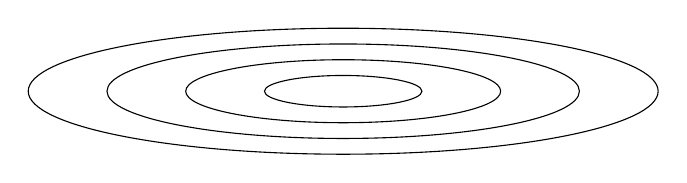
\begin{tikzpicture}
            \draw (0,0) ellipse [x radius=1,y radius=.2];
            \draw (0,0) ellipse [x radius=2, y radius=0.4];
            \draw (0,0) ellipse [x radius=3, y radius=0.6];
            \draw (0,0) ellipse [x radius=4, y radius=0.8];
        \end{tikzpicture}
    \end{figure}
    
\end{xiti}
